As one of the essential model-based approaches, the algorithm of Model-Agnostic Meta-Learning (aka MAML), which was firstly introduced by Finn et al in [3], has been growing more and more popular in the field of meta-learning. As its name implies the approach offers a high compatibility to any model that learns through gradient descent and can handle a variety of problems, including regression, classification as well as policy gradient reinforcement learning.

Just like human can acquire new skills more quickly based on prior experience, the key idea of Model-Agnostic Meta-Learning is training a model for rapid adaptation on new tasks. More specifically, initial parameters of model are trained such that the model can achieve a significant performance on a new task after updating parameters with only a small number of gradient steps, meanwhile avoiding overfitting. Especially it can be readily applied to the popular architectures such as convolutional and recurrent neural networks.

\subsection{ General Model-Agnostic Meta-Learning Algorithm}
Firstly the algorithm is represented in a general form, which is suitable for the problems in various domains, including reinforcement learning. the objective of this approach is to learn an internal feature that is broadly applicable to all tasks in a task distribution $p(\mathcal{T})$
, rather than a single task.

In the context of Model-Agnostic Meta-Learning, a model, that is expected to be able to adapt to a task distribution $p(\mathcal{T})$, is represented by a function $f_{\theta}$ with parameter $\theta$. Generally, a task for meta-learning 
$\mathcal{T}=\left\{\mathcal{L}\left(\mathbf{x}_{1}, \mathbf{a}_{1}, \ldots, \mathbf{x}_{H}, \mathbf{a}_{H}\right) q\left(\mathbf{x}_{1}\right), q\left(\mathbf{x}_{t+1} \mid \mathbf{x}_{t}, \mathbf{a}_{t}\right), H\right\}$ is formed form a loss function $\mathcal{L}$, a distribution over initial observations $q\left(\mathbf{x}_{1}\right)$, a transition distribution $q\left(\mathbf{x}_{t+1} \mid \mathbf{x}_{t}, \mathbf{a}_{t}\right)$, and
an episode length $\mathcal{H}$.

\begin{figure}[H]
	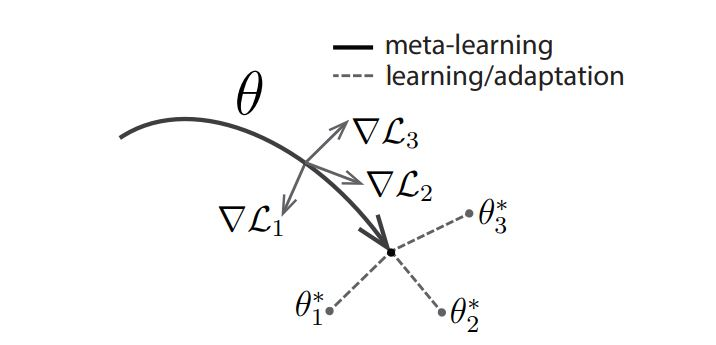
\includegraphics[scale=0.6]{MAML_01.JPG}
	\centering
	\caption{Diagram of model-agnostic meta-learning algorithm (MAML), which optimizes for a representation $\theta$ that can
    quickly adapt to new tasks}
	\label{MAML}
\end{figure}

The key point behind this approach is the transferability of internal representations learned from prior tasks over a distribution $p(\mathcal{T})$. The approach aims to find a set of weights $\theta$ which are more sensitive to specific tasks, by changing the direction of gradient descent, so that the loss on new task can rapidly go down even with a very small number of data.  

\begin{figure}[H]
	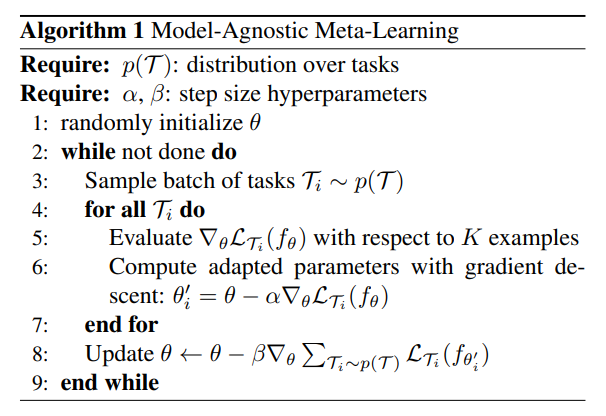
\includegraphics[scale=0.65]{MAML_02.PNG}
	\centering
	\caption{Model-Agnostic Meta-Learning algorithm}
	\label{MAML}
\end{figure}

The principle of the algorithm refers to gradient by gradient,which means two gradient descents are conducted during the meta-training process. When applied to new tasks, the parameters of model $\theta$ become $\theta_{i}^{\prime}$. The updated parameter vector $\theta_{i}^{\prime}$ is computed by doing the first gradient descent on each task $\mathcal{T}_{i}$ among batch of tasks, which is denoted as:

$$\theta_{i}^{\prime}=\theta-\alpha \nabla_{\theta} \mathcal{L}_{\mathcal{T}_{i}}\left(f_{\theta}\right)$$
where $\alpha$ represents step size fixed as hyperparameter and $\mathcal{L}_{\mathcal{T}_{i}}$ is loss of corresponding task.
That is to say, we can get many different updated parameters $\theta_{i}^{\prime}$ on different task $\mathcal{T}_{i}$. Actually the updated weights are not really for update of model, but temporarily used for the second gradient in the outer loop. 

$$
\min _{\theta} \sum_{\mathcal{T}_{i} \sim p(\mathcal{T})} \mathcal{L}_{\mathcal{T}_{i}}\left(f_{\theta_{i}^{\prime}}\right)=\sum_{\mathcal{T}_{i} \sim p(\mathcal{T})} \mathcal{L}_{\mathcal{T}_{i}}\left(f_{\theta-\alpha \nabla_{\theta} \mathcal{L}_{\mathcal{T}_{i}}\left(f_{\theta}\right)}\right)
$$

We can clearly see that the meta-optimization is performed over the
model parameters $\theta$, while the objective is computed using the updated model parameters $\theta_{i}^{\prime}$.

stochastic gradient descent (SGD) is performed in the approach to optimize the parameter of model. Note that here gradient is calculated on the sum of loss over all tasks in the batch of tasks, such that each task do a contribution to the whole model optimization.

$$
\theta \leftarrow \theta-\beta \nabla_{\theta} \sum_{\mathcal{T}_{i} \sim p(\mathcal{T})} \mathcal{L}_{\mathcal{T}_{i}}\left(f_{\theta_{i}^{\prime}}\right)
$$
where $\beta$ is step size specially for the second gradient update.
In general, the first gradient is conducted for obtaining a set of temporary weights, whereas the second gradient descent is for the true update of model parameters. 

\subsection{Model-Agnostic Meta-Learning for Reinforcement Learning}
For conventional reinforcement learning a agent is able to learn rules (or policies) to solve specific problems, but one of the major limitations is that it is unable to generalize the learned policy to newer task. On the contrary, a meta-learning model is expected to adapt to new tasks or new environments that have never been encountered during training. The combination of meta-learning and reinforcement learning, therefore, is of great significance to break the bottleneck of reinforcement learning. A representative example is Model-Agnostic Meta-Learning on reinforcement learning.

Wenn MAML is applied to reinforcement learning, the core idea and the algorithm do not change. The main differences lie in task and loss function. A task in meta-RL consists of  
 an initial state distribution $q_{i}\left(\mathbf{x}_{1}\right)$, a transition distribution $q_{i}\left(\mathbf{x}_{t+1} \mid \mathbf{x}_{t}, \mathbf{a}_{t}\right)$, and the loss function $\mathcal{L}_{\mathcal{T}_{i}}$ corresponds to the reward function $\mathcal{R}$. Instead of images or datapoints tasked in supervised learning, the task of meta-RL is defined as a Markov decision process (MDP), that is composed of a set of states, a set of actions, transition probability function and reward function. We need to notice that it is the policy that is learned as a model which maps from states $\mathbf{x}_{t}$ to actions $\mathbf{a}_{t}$. The loss function for each task ${\mathcal{T}_{i}}$
 is formulized as:
 
 $$\mathcal{L}_{\mathcal{T}_{i}}\left(f_{\phi}\right)=-\mathbb{E}_{\mathbf{x}_{t}, \mathbf{a}_{t} \sim f_{\phi}, q_{\mathcal{T}_{i}}}\left[\sum_{t=1}^{H} R_{i}\left(\mathbf{x}_{t}, \mathbf{a}_{t}\right)\right]
 $$
 
 where ${H}$ is horizon, which indicates  a limited number of sample trajectories in me-RL.
 \begin{figure}[H]
	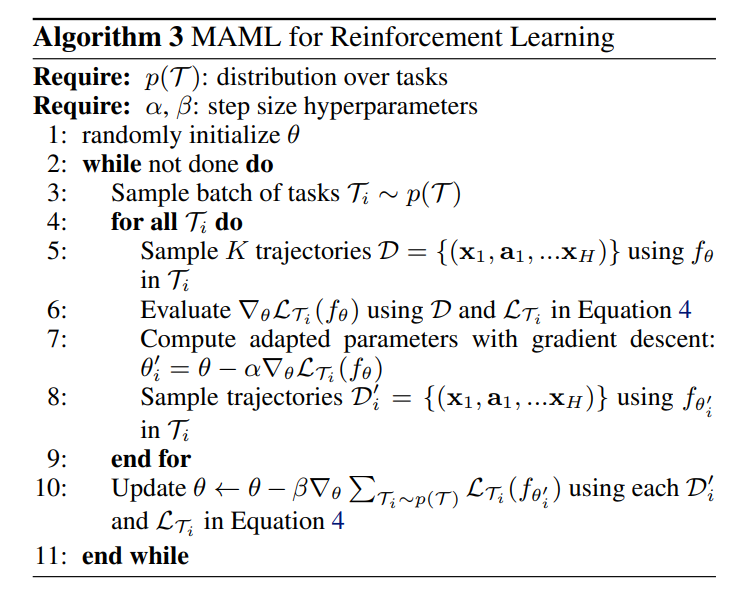
\includegraphics[scale=0.6]{MAML_03.PNG}
	\centering
	\caption{MAML for Reinforcement Learning
}
	\label{MAML}
\end{figure}
In terms of structure, algorithm 3 has no difference with algorithm 1. 
In $K$ -shot reinforcement learning, $K$ trajectories are sampled from the environment, so that the updated parameters $\theta_{i}^{\prime}$ can be calculated by gradient descent. And the second gradient is performed on a new set of trajectories, that leads to real update of model parameters. Additionally, policy gradient methods are used here to estimate two gradients because the reward is not differentiable due to unknown dynamics. 

Several experiments are conducted to evaluate the performance of MAML on reinforcement learning tasks. Among these experiments a neural network policy is trained as model with  two hidden layers of size 100, and ReLU nonlinearities.

The first meta-RL evaluation is in the domain of 2$D$ Navigation, where  a goal position, that a point agent is expected to reach, is chosen randomly in a unit square. The state is the current 2$D$position, and actions correspond to velocity control in the range [−0.1, 0.1]. What's more, the reward is the negative squared distance to the goal. The aim is to maximize the return by training neural network policy with the architecture of MAML.

\begin{figure}[H]
	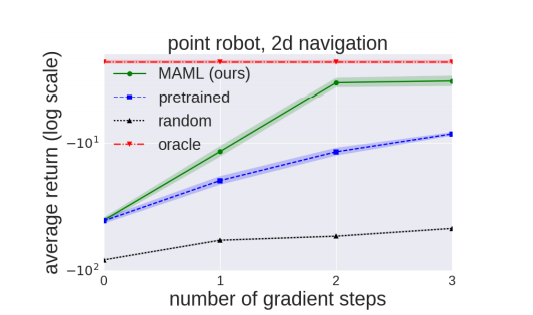
\includegraphics[scale=0.8]{MAML_04.PNG}
	\centering
	\caption{ quantitative results from 2$D$ navigation task}
	\label{MAML}
\end{figure}

The results of four approaches for adaptation on new tasks are showed in Figure 10. They are model that is initialized with MAML, conventional pretraining on the same set of tasks, random initialization, and an oracle policy that receives the goal position as input. We can easily find out that the model learned with MAML obviously outperforms the other three algorithms.

The other more complex evaluation is called locomotion, where two different robots, half  cheetah and ant, run in a particular direction or at a particular velocity. The reward in the goal velocity experiments is the negative absolute value between the current velocity of
the agent and a random goal, while In the goal direction experiments we consider the magnitude of the velocity in either the forward or backward direction as the reward.

\begin{figure}[H]
	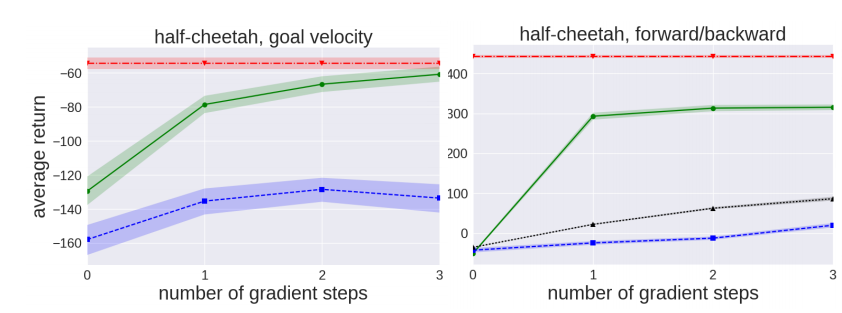
\includegraphics[scale=0.5]{MAML_05.PNG}
	\centering
	\caption{results for the half-cheetah}
	\label{MAML}
\end{figure}

\begin{figure}[H]
	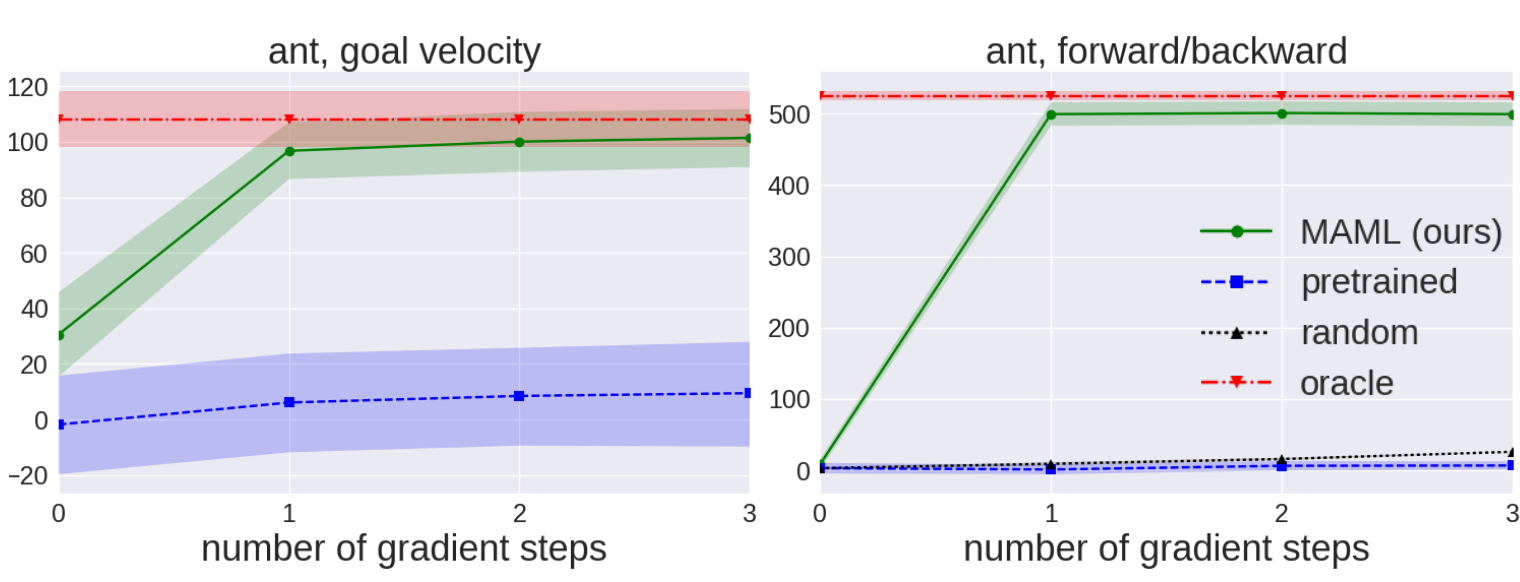
\includegraphics[scale=0.27]{MAML_06.PNG}
	\centering
	\caption{results for the ant}
	\label{MAML}
\end{figure}

From the results we know that the model with MAML performs a faster adaptation on its velocity and direction with a few gradient steps.

Through these two experiments we can draw a conclusion that algorithm MAML can enable faster adaptation on new problems in the field of reinforcement learning. 